\documentclass[letterpaper]{physor2024}

%%% Packages Required by Class (already included)
% fancyhdr
% lastpage
% titling
% titlesec
% ragged2e
% enumitem
% amsmath
% graphicx
% geometry
% newtxtext
% newtxmath
% hyperref
% cleveref
% caption
% authblk
% apptools
% appendix
% ifpdf
% epstopdf

%%% Some other useful packages
% \usepackage{tikz}
% \usepackage{color}
% \usepackage{subcaption}
% \usepackage{algcompatible}
% \usepackage{bm}
% \usepackage{array}

% GLOSSARIES
\usepackage[acronym,nomain,nonumberlist,nogroupskip,nopostdot]{glossaries} % for glossary of acronyms
\setacronymstyle{long-short}
\loadglsentries{glossary}
\makeglossaries
% \renewcommand*{\glstextformat}[1]{\textcolor{black}{#1}} % make glossary color black

% % This file contains custom commands that Lewis uses frequently in LaTeX documents

\usepackage{subcaption}
\usepackage{hyperref}
\hypersetup{colorlinks,allcolors=black}
% % for more https://tex.stackexchange.com/questions/88400/hyperref-changing-the-linkcolor-locally-in-the-toc

% custom equation commands
\newcommand{\QOR}{\qquad \text{OR} \qquad}
\newcommand{\QAND}{\qquad \text{AND} \qquad}
\newcommand{\QTHUS}{\qquad \text{THUS} \qquad}
\newcommand{\QWITH}{\qquad \text{WITH} \qquad}
\newcommand{\QFOR}{\qquad \text{FOR} \qquad}
\newcommand{\QSO}{\qquad \text{SO} \qquad}
\newcommand{\QWHERE}{\qquad \text{WHERE} \qquad}
\newcommand{\QWHEN}{\qquad \text{WHEN} \qquad}
\newcommand{\LINE}{\par\noindent\rule{\textwidth}{0.4pt}\par}
\newcommand{\toinf}{\rightarrow\infty}
\newcommand{\tozero}{\rightarrow0}
\newcommand{\qeq}{\overset{?}{=}}
\newcommand{\ceq}{\overset{\checkmark}{=}}
\newcommand{\Poi}{\text{Poisson}}
\newcommand{\keff}{$k_{e\!f\!f}$}
\newcommand{\kinf}{$k_{\!i\!n\!f}$}
\renewcommand{\epsilon}{\varepsilon} % squiggly epsilon

\def\brac#1{\{#1\}}
\def\Brac#1{\big\{#1\big\}}
\def\BRAC#1{\bigg\{#1\bigg\}}
\def\angbrac#1{\langle#1\rangle}
\def\Angbrac#1{\big\langle#1\big\rangle}
\def\ANGBRAC#1{\bigg\langle#1\bigg\rangle}
\usepackage{float}
\usepackage{multirow} % for special table
% % SI Units
\usepackage{siunitx}
\DeclareSIUnit\n{n}
\DeclareSIUnit\sp{sp}
\title{OpenMC Depletion Analysis of the Virtual Test Bed Gas-Cooled Microreactor}
% \title{Title of the Paper Goes Here: Capitalize the First Letter of Major Words, Centered, 14-Point Times New Roman, on the Second Line from the Top Margin, Not More Than Three Lines Long}

%%% Authors (use arabic numbers: 1, 2, 3, etc. for affiliationNumber)
%%% \addAuthor{GivenName MiddleInitial. FamilyName}{affiliationNumber}
\addAuthor[ligross@wissc.edu]{Lewis I. Gross}{1}
\addAuthor{Paul P.~H. Wilson}{1}

%%% Affiliations (from authblk)
%%% \addAffiliation{affiliationNumber}{Name of Institute, City, State/Country}
\addAffiliation{1}{University of Wisconsin - Madison, Madison, Wisconsin}

%%% Write text for abstract
%%% Most text modifying commands will work in abstract
\Abstract{OpenMC is a state-of-the art, \gls{os} Monte Carlo transport code. This work uses OpenMC for depletion analysis of the \gls{vtb} \gls{gcmr}. This microreactor features a prismatic, \gls{triso}-fueled, gas-cooled for an infinite-assembly model. Since this reactor is intended for load-following, a depletion analysis was run at 100\%, 50\%, and 10\% of the rated power (225 kWt) for both explicitly represented \gls{triso} and volume-homogenized fuel. The time steps used were twice as long and ten times as long for the lower power cases, respectively, to ensure the same total burnup occurred at each time step. The isotopics after one year of operation at steady-state were compared at each power for both fidelities.}

%%% List up to 5 keywords separated by a comma
\keywords{OpenMC, TRISO, depletion, microreactor, gas-cooled}

%%% Provide a short title for the header on odd pages
\shortTitle{Depletion of a TRISO Fueled, Gas-Cooled Microreactor }

%%% Provide a short author listing for the header on even pages
\authorHead{Gross and Wilson}

%%% If LaTeX reports the line number of an error at \begin{document} it
%%%   is most likely due to an error in one of the commands above
\begin{document}

\section{INTRODUCTION}\label{sec:intro}
For advanced reactors, especially those in the early stages, sufficient \gls{ms} is required to ensure the success of the design concept. The \gls{vtb} \cite{vtb2023} is a repository of reactor models used for research and demonstration of current tools in the nuclear industry as a part of the \gls{neams} initiative. Various types of reactors are available on the \gls{vtb}; microreactors are one viable class of next generation systems. [TODO add microreactor refs as appropriate]

% M&S -> VTB -> MICROREACTORS -> GCMR -> previous GCMR work

\section{DEPLETION THEORY}\label{sec:depletion}

\section{SYSTEM DESCRIPTION}\label{sec:system}
The system analyzed is based from the \gls{vtb} \gls{gcmr}. \cref{fig:vtb_gcmr} shows a diagram of the system.
\cite{openmc}

\begin{figure}[H]
    \centering
    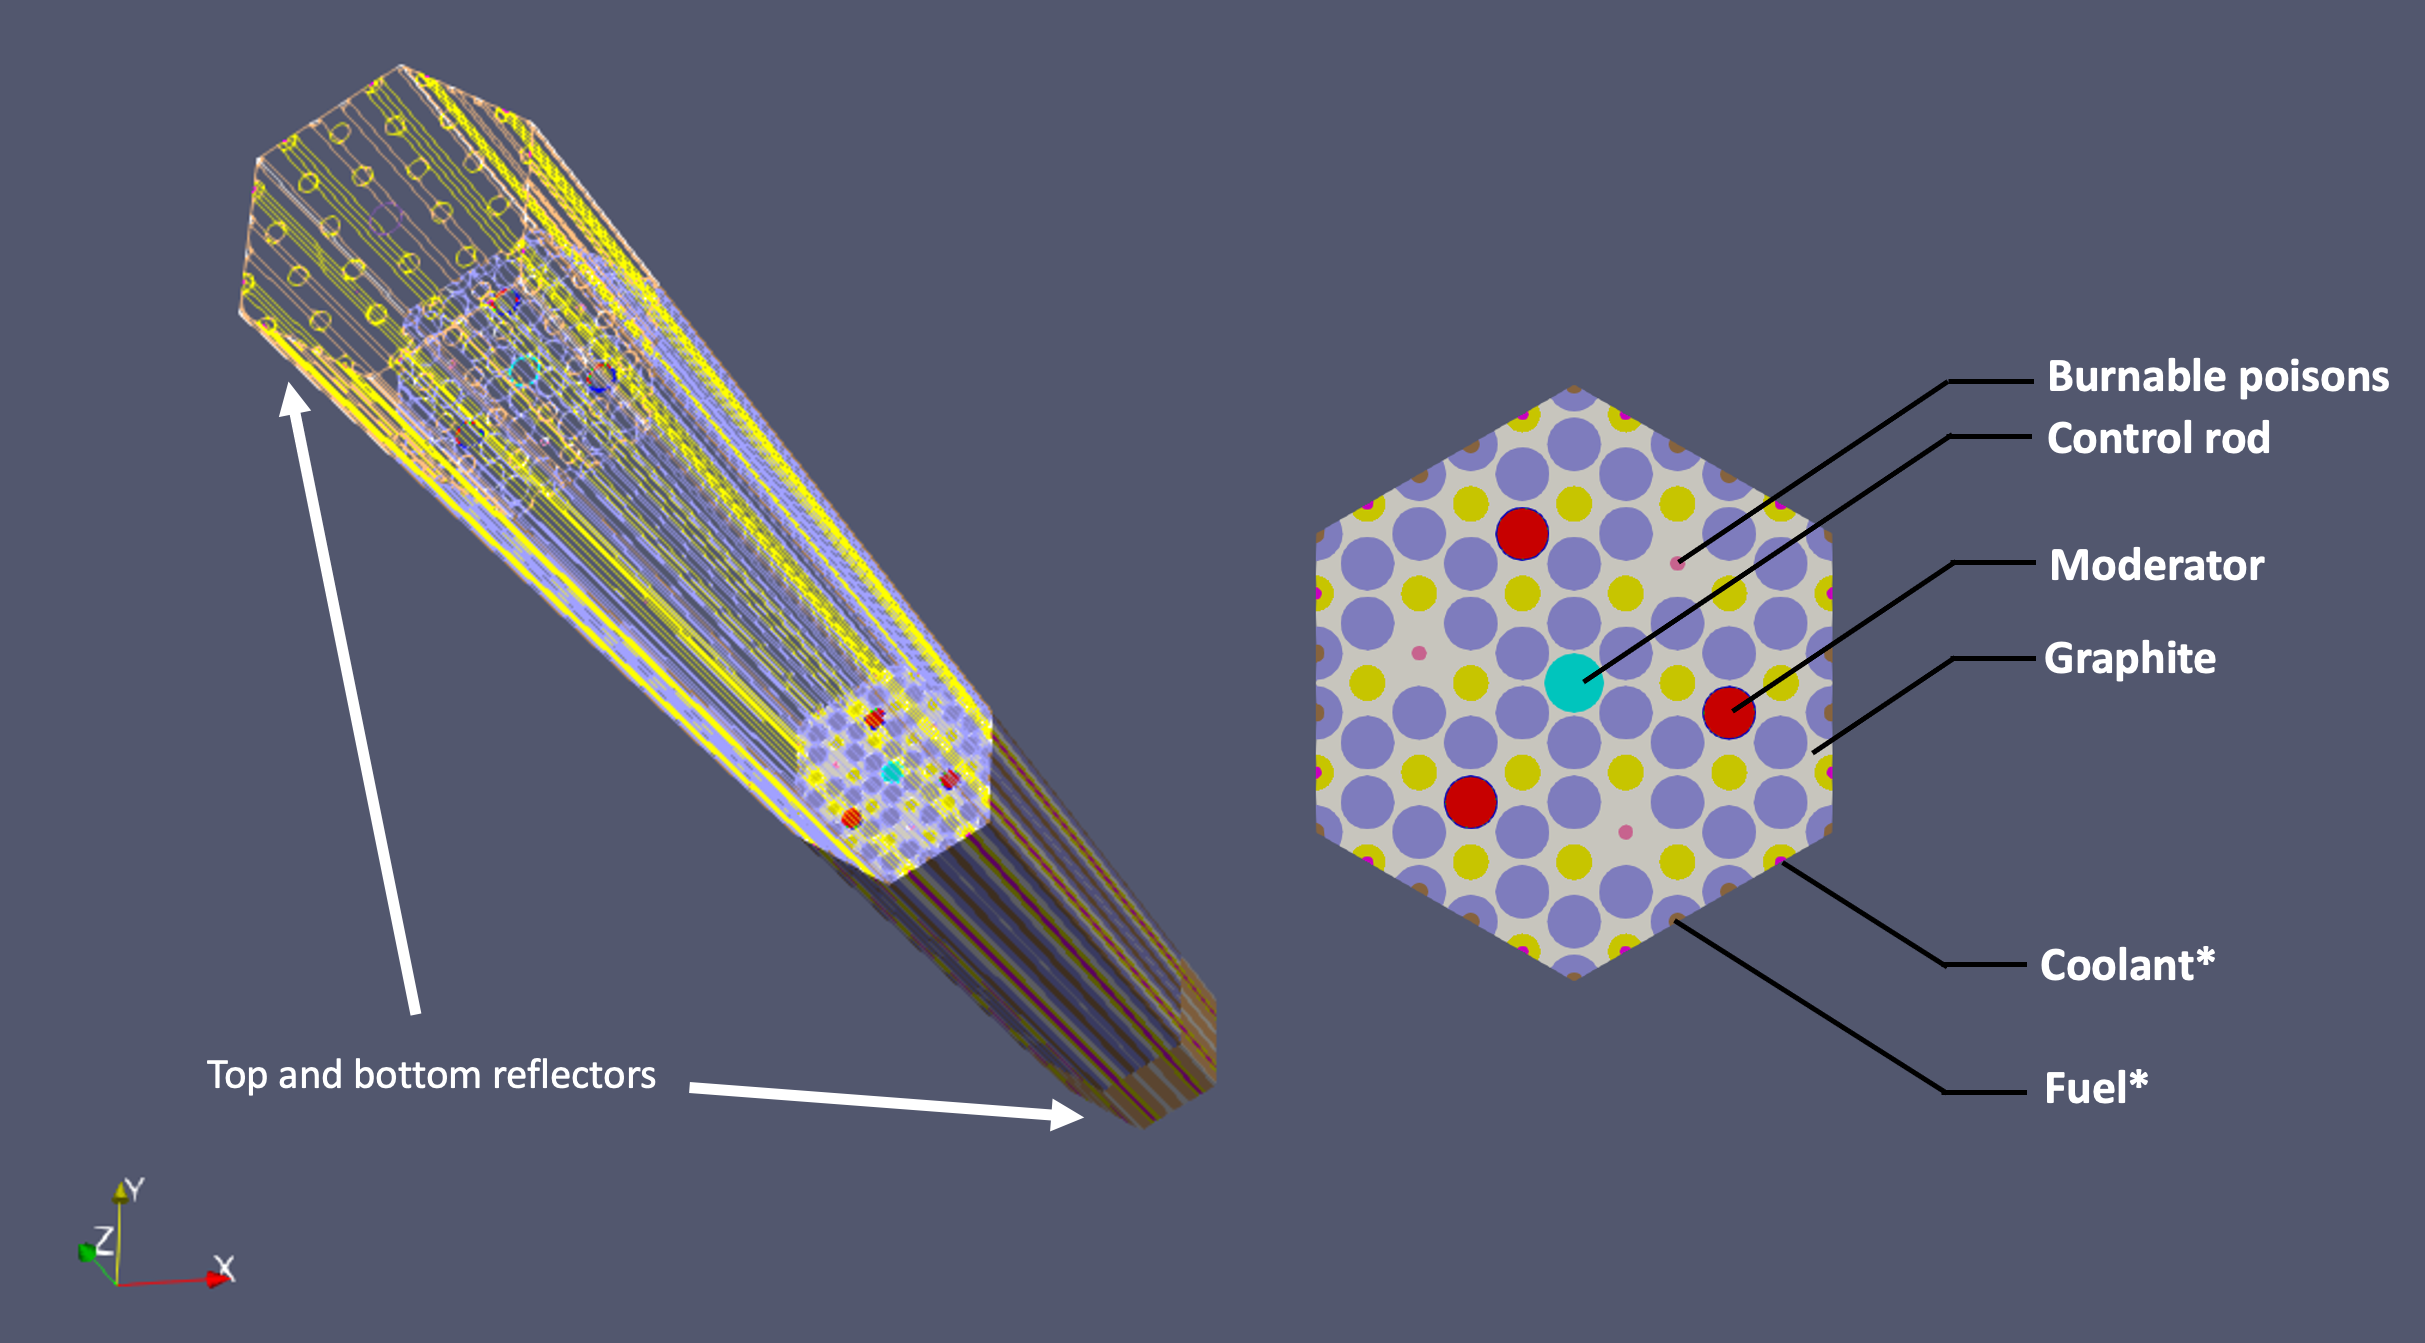
\includegraphics[width=\linewidth]{figures/vtb_gcmr_diagram.jpg}
    \caption{An image of the \gls{vtb} \gls{gcmr} along with a cross section of the fuel containing section of the system.}
    \label{fig:vtb_gcmr}
\end{figure}


\section{OPENMC MODEL}\label{sec:openmc_model}


\section{RESULTS}\label{sec:results}
Present results.

\section{CONCLUSIONS}\label{sec:conclusions}
Present summary and conclusions here

\section*{ACKNOWLEDGEMENTS}
Acknowledge the help of colleagues, and sources of funding, as appropriate.

The first author was supported in part by the US Nuclear Regulatory Commission's Graduate Fellowship Program administered by the University of Wisconsin-Madison.

\printglossaries

\bibliographystyle{physor2024}
\bibliography{physor2024}

\appendix

\section{}
If necessary, include Appendices numbered in upper case alphabetical order.

To ensure a uniform, professional look at the proceedings, please only modify the format of this template after checking with the publication chair first.


\end{document}